\documentclass[conference]{IEEEtran}
\IEEEoverridecommandlockouts
% The preceding line is only needed to identify funding in the first footnote. If that is unneeded, please comment it out.
\usepackage{cite}
\usepackage{amsmath,amssymb,amsfonts}
\usepackage{algorithmic}
\usepackage{graphicx}
\usepackage{textcomp}
\usepackage{xcolor}
\usepackage{subfigure}
\usepackage{url}
\usepackage{soul}
\usepackage{fancyhdr}

\usepackage[algo2e,vlined,ruled]{algorithm2e}

\usepackage[colorlinks, linkcolor=red, anchorcolor=blue, citecolor=green]{hyperref}

\pagestyle{fancy}
\cfoot{\thepage}


\def\BibTeX{{\rm B\kern-.05em{\sc i\kern-.025em b}\kern-.08em
    T\kern-.1667em\lower.7ex\hbox{E}\kern-.125emX}}
\begin{document}

\title{MDS5210: Machine Learning Final project—Robust Matrix Factorization
\\
% {\footnotesize \textsuperscript{*}Note: Sub-titles are not captured in Xplore and
% should not be used}

}

\author{\IEEEauthorblockN{\textbf{Peng Deng}}
\IEEEauthorblockA{School of Data Science \\
\texttt{{220041042}}}
\and
\IEEEauthorblockN{\textbf{Shihan Wang}}
\IEEEauthorblockA{School of Data Science \\
\texttt{{220041083}}}
\and
\IEEEauthorblockN{\textbf{Han Yang}}
\IEEEauthorblockA{School of Data Science \\
\texttt{{220041046}}}
\and
\IEEEauthorblockN{\textbf{Jing Sun}}
\IEEEauthorblockA{School of Data Science \\
\texttt{{116010199}}}
\and
\IEEEauthorblockN{\textbf{Sicheng Liu}}
\IEEEauthorblockA{School of Data Science \\
\texttt{{220041011}}}
\and
}

\maketitle
\thispagestyle{fancy}
\cfoot{\thepage}
\renewcommand{\thefootnote}{\fnsymbol{footnote}}
\begin{abstract}
This paper\footnote[1]{
	Group Member and Responsibilities:\\
	Peng Deng: A-IRLS Algorithm, Data Processing, Result Generation\\
	Shihan Wang: Subgradient method, Data Generation\\
	Han Yang: A-IRLS Algorithm, Report Writing\\
	Jing Sun: Subgradient method, Slides Making\\
	Sicheng Liu: A-IRLS Algorithm, Report Writing} is about the application of subgradient method and A-IRLS algorithms to solve the optimization problem of matrix factorization/PCA and apply them into different situations. 
We first evaluate our algorithms on artificially generated dataset to validate their effectiveness. Then we move to the real dataset and apply the model on the problem of face shadow removal and video frames static background extraction. And we found that both algorithms provide satisfactory performance while A-IRLS algorithm reaches smaller error and converges in much faster speed while subgradient method has much shorter running time.\footnote[2]{\url{https://github.com/Dpaul891/Machine_Learning_Project}}



\end{abstract}

\begin{IEEEkeywords}
Machine Learning, PCA, Sungradient, A-IRLS
\end{IEEEkeywords}
\section{Introduction}
PCA/matrix factorization is a very useful and popular method in the field of computer vision. In our project, we will adopt this method and build a machine learning system to solve the problem of removing the shadow of face images and extracting backgrounds form video frames.

PCA/matrix factorization aims to factorize the data matrix $\boldsymbol{X}\in\mathbb{R}^{d\times n}$ into $\boldsymbol{U}\boldsymbol{V}^{\top}$. The underlying idea for applying low-rank matrix factorization is that the data matrix $\boldsymbol{X}$ possesses intrinsically low-rank structures. Under the sparsity assumption of the residual error, one possible learning problem formulation is as formula (\ref{eq1}).
\begin{equation}
    \label{eq1}
    \underset{\boldsymbol{U} \in \mathbb{R}^{d \times r}, \boldsymbol{V} \in \mathbb{R}^{n \times r}}{\operatorname{minimize}}\left\|\boldsymbol{X}-\boldsymbol{U} \boldsymbol{V}^{\top}\right\|_{0}
\end{equation}
Assume that $\boldsymbol{X}=\boldsymbol{L}^{\star} + \boldsymbol{S}^{\star}$, $\boldsymbol{L}^{\star}$ is a low-rank matrix with rank $r\ll\text{min}\left(d,n\right)$ and $\boldsymbol{S}^{\star}\in\mathbb{R}^{d\times n}$ is a sparse matrix (the residual error). $\boldsymbol{L}^{\star}$ can be factorized as $\boldsymbol{L}^{\star}=\boldsymbol{U}^{\star}\boldsymbol{V}^{\star\top}$, where $\boldsymbol{U}^{\star}\in\mathbb{R}^{d\times r}$, $\boldsymbol{V}^{\star}\in\mathbb{R}^{n\times r}$. Thus, our goal is equivalent to find the underlying $\boldsymbol{U}^{\star}$ and $\boldsymbol{V}^{\star}$ given $\boldsymbol{X}$. Plugging $\boldsymbol{U}^{\star}$ and $\boldsymbol{V}^{\star}$ into (\ref{eq1}), we get $\|\boldsymbol{S}^{\star}\|_0$. The fact that $\boldsymbol{S}^{\star}$ is sparse, together with the sparsity promoting nature
of $l_0$-quasinorm, suggests that $\left(\boldsymbol{U}^{\star},\boldsymbol{V}^{\star}\right)$ is likely to be one optimal solution of (\ref{eq1}). Thus, solving (\ref{eq1}) to the globally optimal solution is likely to provide us the underlying $\left(\boldsymbol{U}^{\star},\boldsymbol{V}^{\star}\right)$.
However, the $l_0$-quasinorm makes the learning problem (\ref{eq1}) intractable, so that we use the $l_1$-norm to replace the $l_0$-quasinorm and the final tractable learning problem is as formula (\ref{for_1_norm}).
\begin{equation}
    \label{for_1_norm}
    \underset{\boldsymbol{U} \in \mathbb{R}^{d \times r}, \boldsymbol{V} \in \mathbb{R}^{n \times r}}{\operatorname{minimize}}\left\|\boldsymbol{X}-\boldsymbol{U} \boldsymbol{V}^{\top}\right\|_{1}
\end{equation}



In our project, we will implement \textbf{subgradient method} and \textbf{alternating iteratively reweighed least squares (A-IRLS)} algorithms to solve the learning problem.


\section{Algorithms Description}
\subsection{Subgradient Method}
The loss function $\mathcal{L}=\|\boldsymbol{X}-\boldsymbol{U} \boldsymbol{V}^{\top}\|_{1}$ is not differentiable and we cannot employ gradient descent method directly. Thus, we apply subgradient method to solve the problem. We first calculate the subgradient at $\boldsymbol{U}$ and $\boldsymbol{V}$:
\begin{equation}
    \label{eq2}
	\begin{split}
		\partial \mathcal{L}(\boldsymbol{U})&=-\operatorname{sign}(\boldsymbol{X}-\boldsymbol{U} \boldsymbol{V}^{\top})\boldsymbol{V}\\
		\partial \mathcal{L}(\boldsymbol{V})&=-\operatorname{sign}(\boldsymbol{X}-\boldsymbol{U} \boldsymbol{V}^{\top})^{\top}\boldsymbol{U} 
	\end{split}
\end{equation}
Then set an initial $\alpha$ and use diminishing stepsize, so in each iteration, we have:
\begin{equation}
	\begin{split}
		\boldsymbol{U}_{k+1}&=\boldsymbol{U}_{k}-\cfrac{\alpha}{\sqrt n}\cdot\partial\mathcal{L}(\boldsymbol{U}_{k})\\
		\boldsymbol{V}_{k+1}&=\boldsymbol{V}_{k}-\cfrac{\alpha}{\sqrt n}\cdot\partial\mathcal{L}(\boldsymbol{V}_{k})
	\end{split}
    \label{eq4}
\end{equation}
After certain iteration, we can obtain the final estimation of $\left(\boldsymbol{U}^{\star},\boldsymbol{V}^{\star}\right)$ as $\left(\widehat{\boldsymbol{U}},\widehat{\boldsymbol{V}}\right)$.

The subgradient method to solve this learning problem can be summarized as Algorithm (\ref{alg:subgradient}).
\begin{algorithm2e}[h]
\caption{\textbf{The Subradient Method}}    
\label{alg:subgradient}
\lnlset{alg:fis-1}{1}{Initialization: Choose $\boldsymbol{U}_{0} \in \mathbb{R}^{d\times r}, \boldsymbol{V}_{0} \in \mathbb{R}^{n\times r}$ with $\boldsymbol{U}_{0}^{(i,j)}\sim N\left(0,1\right), \boldsymbol{V}_{0}^{(i,j)}\sim N\left(0,1\right)$}. Choose $\alpha$. \\ 
\For{$k = 0,1,2,\cdots,N$}{
\lnlset{alg:pi-2}{2}{Update $\boldsymbol{U}$ and $\boldsymbol{V}$: \quad \quad $\boldsymbol{U}_{k+1}=\boldsymbol{U}_{k}-\cfrac{\alpha}{\sqrt n}\cdot\partial\mathcal{L}(\boldsymbol{U}_{k})$ $\boldsymbol{V}_{k+1}=\boldsymbol{V}_{k}-\cfrac{\alpha}{\sqrt n}\cdot\partial\mathcal{L}(\boldsymbol{U}_{k})$} \\
} 
\Return{$\left(\boldsymbol{U}_{N},\boldsymbol{V}_{N}\right)$}
\end{algorithm2e}
	

\subsection{A-IRLS Algorithm}
The method of Alternating iteratively reweighed least squares (A-IRLS) is used to solve certain optimization problems in the form of $p$-norm iteratively in which every iteration involves solving a subproblem of weighted least squares\cite{A-IRLS}.

Specifically, in our project $p=1$ and in each step, we should fix $\boldsymbol{U}$ and $\boldsymbol{V}$ respectively and solve the weighted least squares problem of another variable. Thus, in each iteration:
\begin{equation}
    \label{eq6}
	\begin{split}
		\boldsymbol{V}_{k+1}(i,:)&=(\boldsymbol{U}_{k}^{\top}\boldsymbol{W}^{(v,i)}_{k}\boldsymbol{U}_{k})^{-1}\boldsymbol{U}_{k}^{\top}\boldsymbol{W}^{(v,i)}_{k}\boldsymbol{X}(:,i)\\
		\boldsymbol{U}_{k+1}(i,:)&=(\boldsymbol{V}_{k+1}^{\top}\boldsymbol{W}^{(u,i)}_{k}\boldsymbol{V}_{k+1})^{-1}\boldsymbol{V}_{k+1}^{\top}\boldsymbol{W}^{(u,i)}_{k}\boldsymbol{X}^{\top}(:,i)\\
	\end{split}
\end{equation}
where $\boldsymbol{W}_k^{(u,i)}$ and $\boldsymbol{W}_k^{(v,i)}$ are the diagonal matrix of weights at the $k^{th}$ iteration for $\boldsymbol{U}\left(i,:\right)$ and $\boldsymbol{V}\left(i,:\right)$ respectively. They are initialized with $\boldsymbol{W}^{(u,i)}_{0}=\boldsymbol{I}_n; \boldsymbol{W}^{(v,i)}_{0}=\boldsymbol{I}_d$. Let $\delta$ be some small value like $0.0001$ then the update formula is:
\begin{equation}
    \label{eq8}
	\begin{split}
		\boldsymbol{W}^{(u,i)}_{k}&=\operatorname{diag}\left(\cfrac{1}{\operatorname{max}\{\delta, |\boldsymbol{X}^{\top}(:,i)-\boldsymbol{V}_{k}\boldsymbol{U}_{k}(i,:)|\}}\right)\\
		\boldsymbol{W}^{(v,i)}_{k}&=\operatorname{diag}\left(\cfrac{1}{\operatorname{max}\{\delta, |\boldsymbol{X}(:,i)-\boldsymbol{U}_{k}\boldsymbol{V}_{k}(i,:)|\}}\right)
	\end{split}
\end{equation}
The A-IRLS Algorithm to solve this learning problem can be summarized as Algorithm (\ref{alg:A-IRLS}).
\begin{algorithm2e}[h]
\caption{\textbf{The A-IRLS Algorithm}}    
\label{alg:A-IRLS}
\lnlset{alg:fis-1}{1}{Initialization: Choose $\boldsymbol{U}_{0} \in \mathbb{R}^{d\times r}, \boldsymbol{V}_{0} \in \mathbb{R}^{n\times r}$ with $\boldsymbol{U}_{0}^{(i,j)}\sim N\left(0,1\right), \boldsymbol{V}_{0}^{(i,j)}\sim N\left(0,1\right)$}. Choose $\boldsymbol{W}^{(u,i)}_{0}=\boldsymbol{I}_n; \boldsymbol{W}^{(v,i)}_{0}=\boldsymbol{I}_d$. Choose $\delta=0.0001.$ \\ 
\For{$k = 0,1,2,\cdots,N$}{
\lnlset{alg:pi-2}{2}{Fix $\boldsymbol{U}_k$ and update $\boldsymbol{V}_{k+1}$: \quad } \\
\For{$i=0,1,2,\cdots,n$}{
{\small	$\boldsymbol{V}_{k+1}(i,:)=(\boldsymbol{U}_{k}^{\top}\boldsymbol{W}^{(v,i)}_{k}\boldsymbol{U}_{k})^{-1}\boldsymbol{U}_{k}^{\top}\boldsymbol{W}^{(v,i)}_{k}\boldsymbol{X}(:,i)$\qquad\qquad\qquad\qquad\qquad\qquad\qquad
	$\boldsymbol{W}^{(v,i)}_{k}=\operatorname{diag}\left(\cfrac{1}{\operatorname{max}\{\delta, |\boldsymbol{X}(:,i)-\boldsymbol{U}_{k}\boldsymbol{V}_{k}(i,:)|\}}\right)$}
}
\lnlset{alg:pi-3}{3}{Fix $\boldsymbol{V}_{k+1}$ and update $\boldsymbol{U}_{k+1}$: \quad} \\
\For{$i=0,1,2,\cdots,d$}{
{\small	$\boldsymbol{U}_{k+1}(i,:)=(\boldsymbol{V}_{k+1}^{\top}\boldsymbol{W}^{(u,i)}_{k}\boldsymbol{V}_{k+1})^{-1}\boldsymbol{V}_{k+1}^{\top}\boldsymbol{W}^{(u,i)}_{k}\boldsymbol{X}^{\top}(:,i)$
$\boldsymbol{W}^{(u,i)}_{k}=\operatorname{diag}\left(\cfrac{1}{\operatorname{max}\{\delta, |\boldsymbol{X}^{\top}(:,i)-\boldsymbol{V}_{k}\boldsymbol{U}_{k}(i,:)|\}}\right)$}
}
} 
\Return{$\left(\boldsymbol{U}_{N},\boldsymbol{V}_{N}\right)$}
\end{algorithm2e}







\section{Evaluation on Artificial Dataset}
In this part, we evaluate our algorithms on artificially generated dataset. We first generate the underlying low-rank matrix $\boldsymbol{L}^{\star}=\boldsymbol{U}^{\star}\boldsymbol{V}^{\star\top}$ by generating $\boldsymbol{U}^{\star}\in\mathbb{R}^{d\times r}$, $\boldsymbol{V}^{\star}\in\mathbb{R}^{n\times r}$ with $i.i.d.$ standard Gaussian entries. To generate $\boldsymbol{S}^{\star}\in\mathbb{R}^{d\times n}$ we first randomly select $pdn$ locations. Then, we fill each of the selected locations with an $i.i.d.$ mean 0 and variance 100 Gaussian entry, while the remaining locations are set to 0. Here $p$ is the ratio of the nonzero elements in $\boldsymbol{S}^{\star}$ that represent the sparsity of the residual error.

We set $d=n=50$, $r=5$ and first set $p=0.3$ to run the two algorithms on data $\boldsymbol{X}$ to plot the error $\|\boldsymbol{U}_k\boldsymbol{V}_k^{\top}-\boldsymbol{L}^{\star}\|_F$ in the process of iteration. After that, we vary $p\in\left\{0.1,0.2,0.3,\cdots,0.8\right\}$ and run algorithms on $\boldsymbol{X}$ with different $p$ and plot the final error $\|\widehat{\boldsymbol{U}}\widehat{\boldsymbol{V}}^{\top}-\boldsymbol{L}^{\star}\|_F$ for each algorithm to compare the performance under different sparsity of residual errors $\boldsymbol{S}^{\star}$. The results are shown below:

\subsection{Subgradient Method}
\begin{figure}[htbp]
  \centering
  \subfigure[Iterated errors of Subgradient with $p=0.3$]{\label{sub1}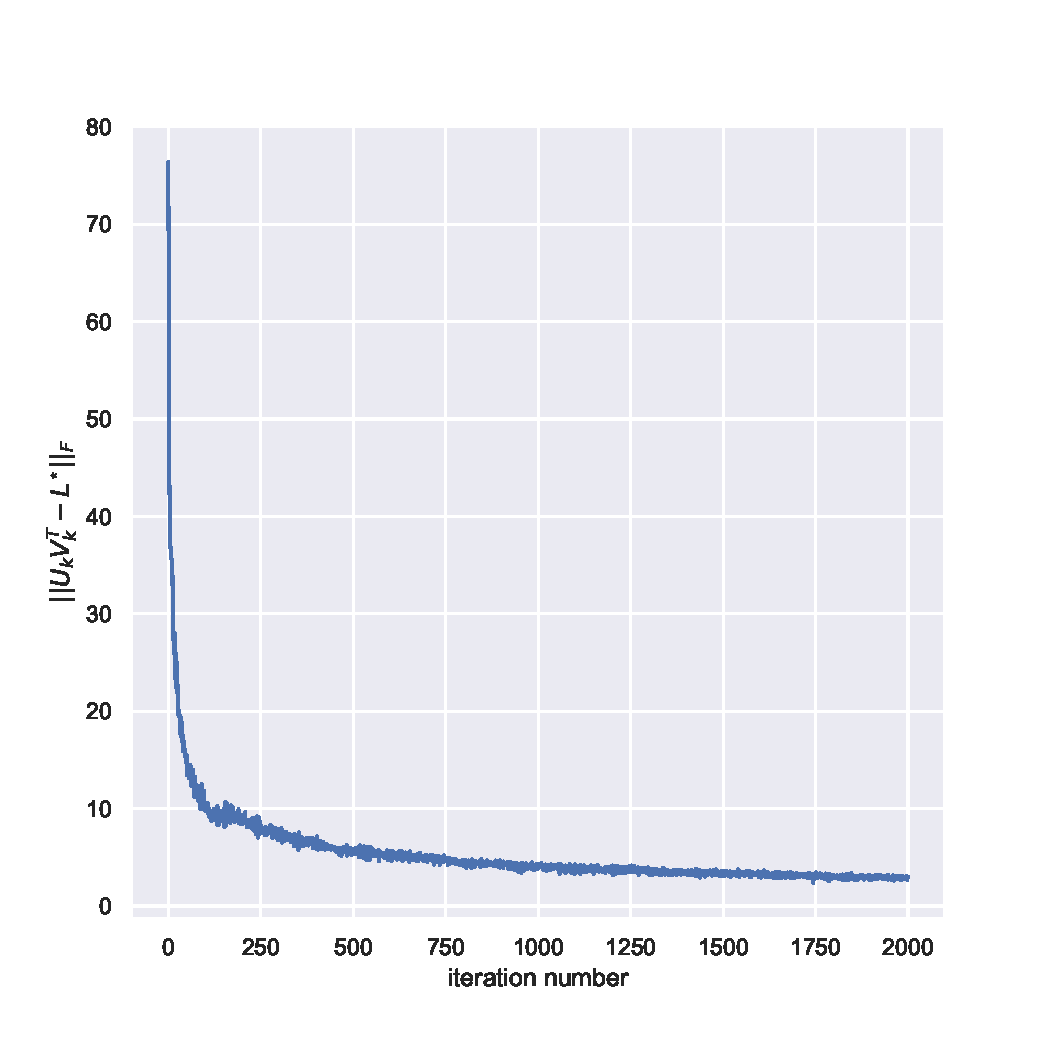
\includegraphics[width=0.47\linewidth]{image/Figure 1 Subgradient}}
  \quad
  \subfigure[Final errors of Subgradient with different $p$]{\label{sub2}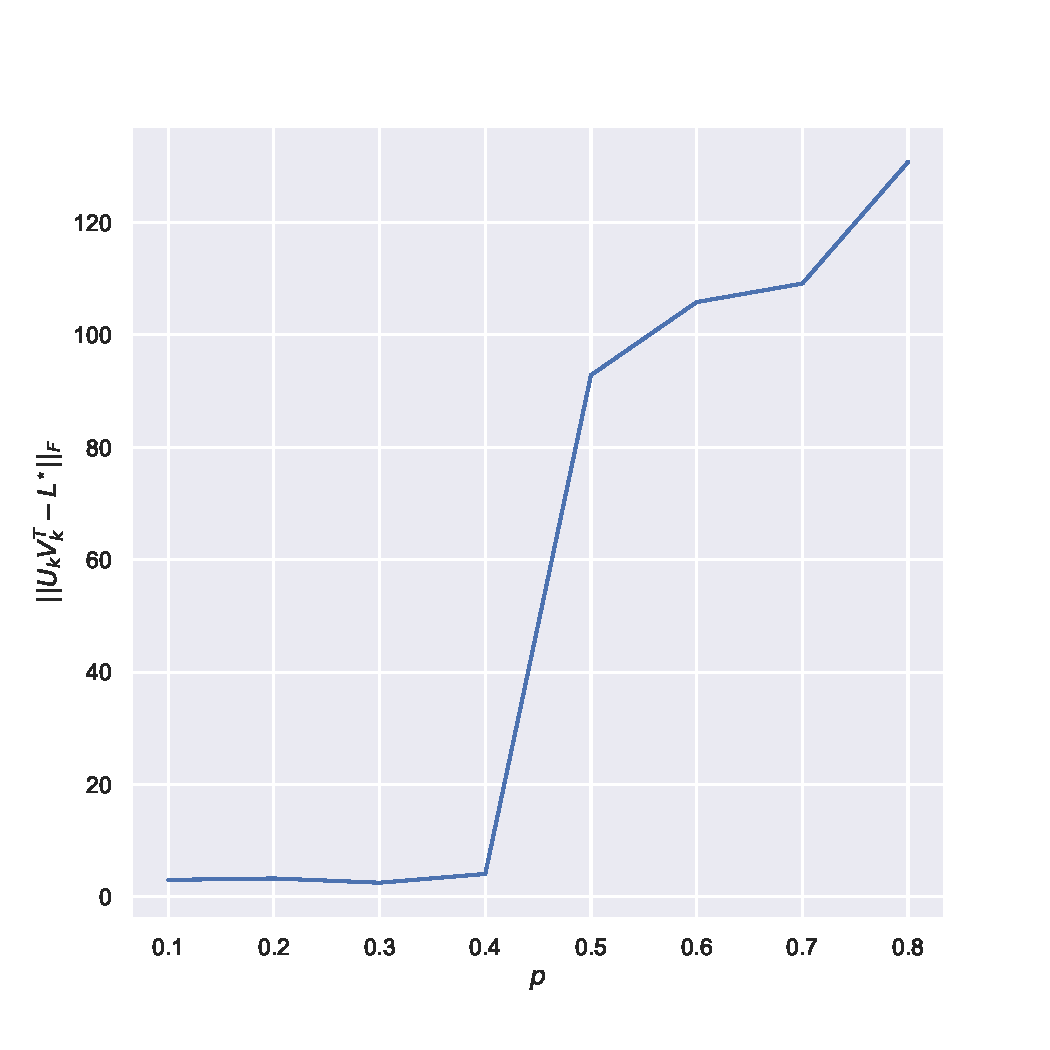
\includegraphics[width=0.47\linewidth]{image/Figure 2 Subgradient}}
  \caption{The subgradient method}
  \label{sub}
\end{figure}

From Figure \ref{sub1}, we found that the error of sub-gradient method will decrease rapidly during first 250 iterations and the rate of descent will be slower in the following iterations. Finally, the error will fluctuate around 3.

Based on Figure \ref{sub2}, the final error will generally increase when $p$ increases. When $p$ ranges from 0.1 to 0.4, the achieved error is near 0 which is satisfactory. When $p$ is larger than 0.4, the final error will increase a lot. This is because when $p$ is larger, the matrix $\boldsymbol{S}^{\star}$ is not sparse, so the algorithm is not suitable at this moment.
\subsection{A-IRLS Algorithm}

\begin{figure}[htbp]
    \centering
    \subfigure[Iterated errors of A-IRLS with $p=0.3$]{\label{airls1}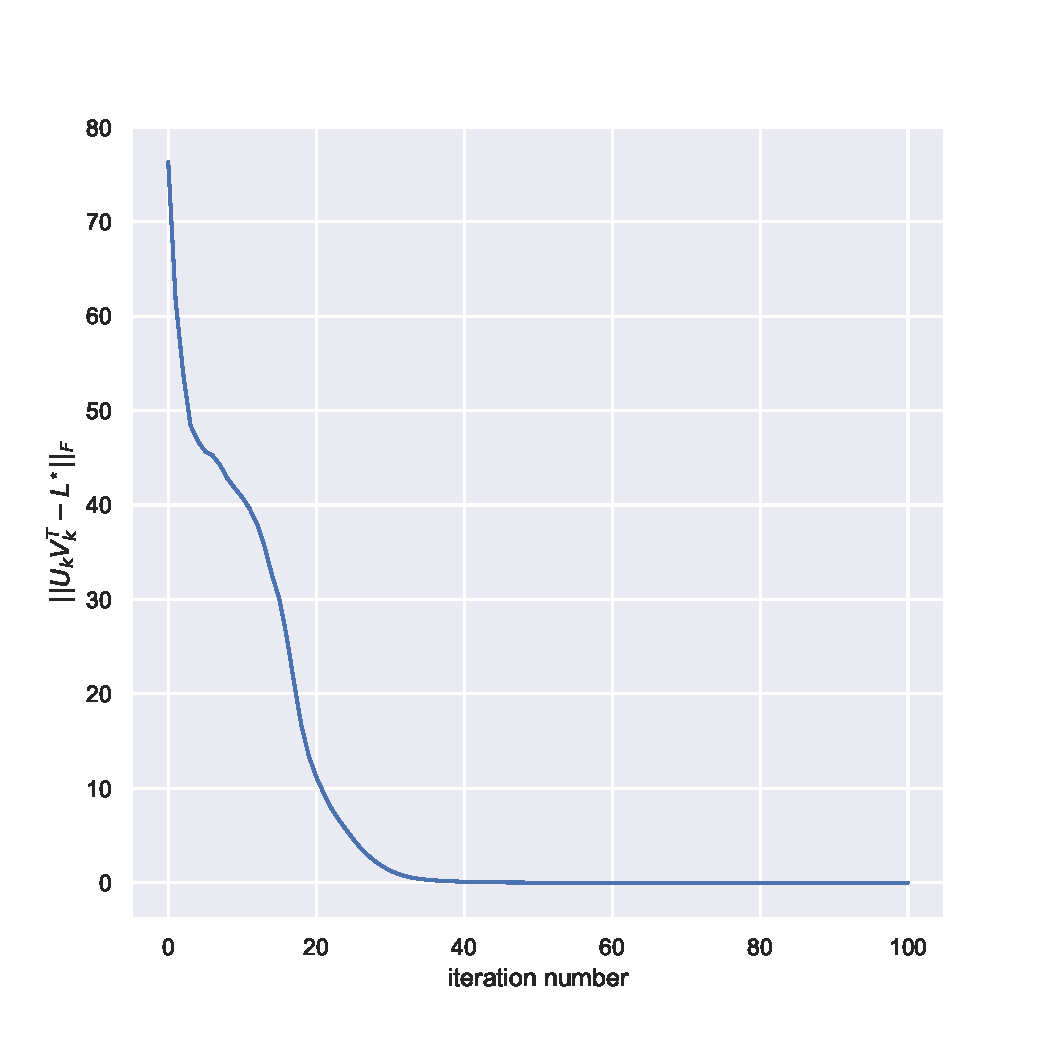
\includegraphics[width=0.47\linewidth]{image/Figure 3 A-IRLS}}
    \quad
    \subfigure[Final errors of A-IRLS with different $p$]{\label{airls2}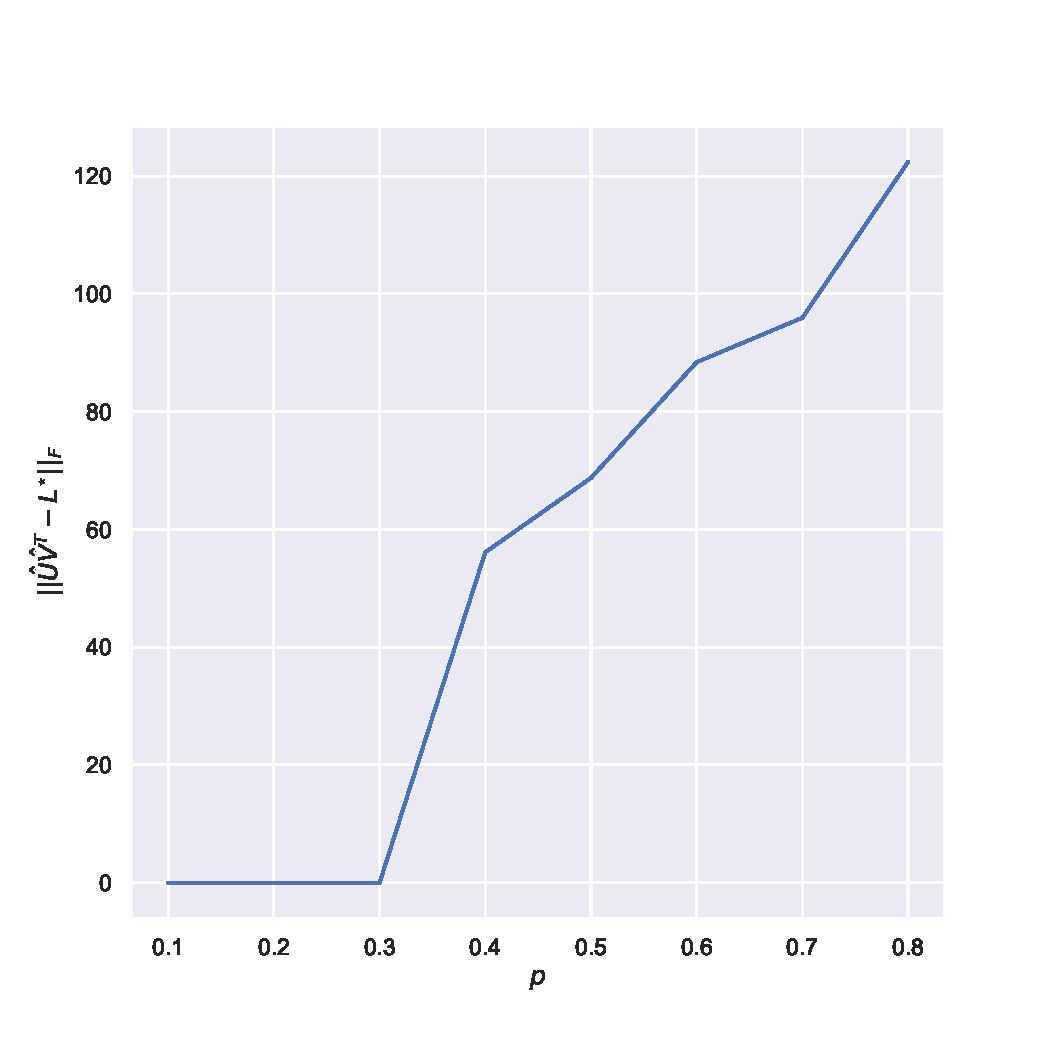
\includegraphics[width=0.47\linewidth]{image/Figure 4 A-IRLS}}
    \caption{The A-IRLS method}
    \label{airls}
  \end{figure}

As shown in Figure \ref{airls1}, the error of A-IRLS algorithm reaches 0 in the $60^{th}$ iteration which is much faster than sub-gradient method. 

From Figure \ref{airls2}, we found that when $p$ ranges from 0.1 to 0.3, the final error will achieve 0 in the first 100 iterations and the error will increase a lot when $p$ is larger than 0.3, which is very similar to the sub-gradient method.

According to the iterated errors plot, we can see that both algorithms have successfully made the errors decrease while the descent speed of A-IRLS is much better. And from the final errors plot, we can conclude that both algorithms perform well when $p$ ranges from 0.1 to 0.3.

\section{Shadow and Illumination Removing}
Next, we will apply our two algorithms on the Yale-B02 face image dataset to remove the shadow and illumination. The main idea is that the clean face images of the same person are similar to each other such that they can form a low-rank matrix (regard each face image as one column), while the illumination and shadow is sparse. The results are shown below:

\subsection{Subgradient Method}
We set the iteration number equals to 2000 to get $\boldsymbol{L}^{\star}=\boldsymbol{U}^{\star}\boldsymbol{V}^{\star\top}$ and we can see that the loss decreases quickly in the first 250 iterations and then fluctuates around a value in later iterations as in Figure \ref{sub_face}.

\begin{figure}[htbp]
	\centering
	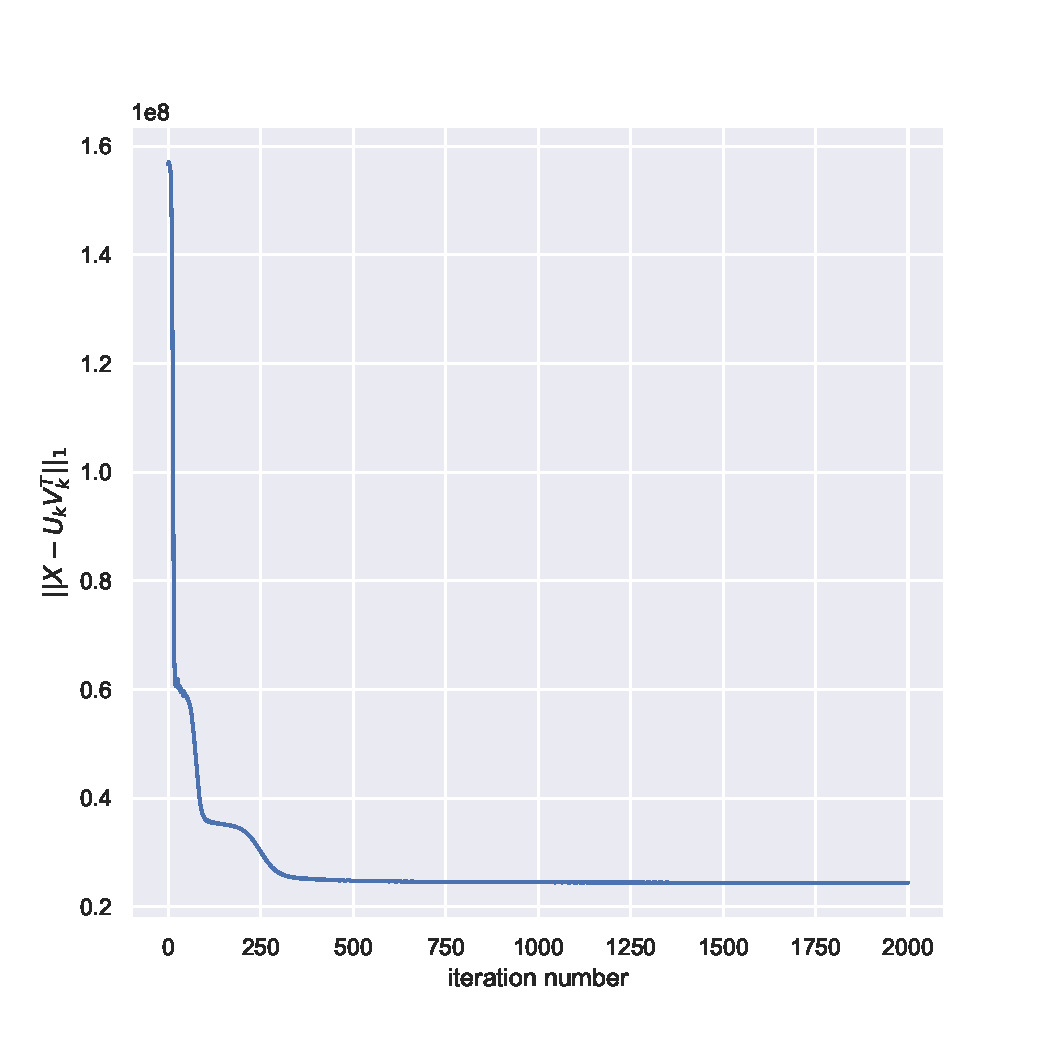
\includegraphics[width=0.6\linewidth]{image/Figure 5 Subgradient}
	\caption{Iteration Process of Subgradient in Face Image Data}
	\label{sub_face}
\end{figure}

The results of face shadow removal are shown as Figure \ref{sub_face1}. $\boldsymbol{X}$ is the original images, $\boldsymbol{\widehat{L}}$ is the processed images and $\boldsymbol{\widehat{S}}$ is the removed shadow. 
\begin{figure}[htbp]
	\centering
	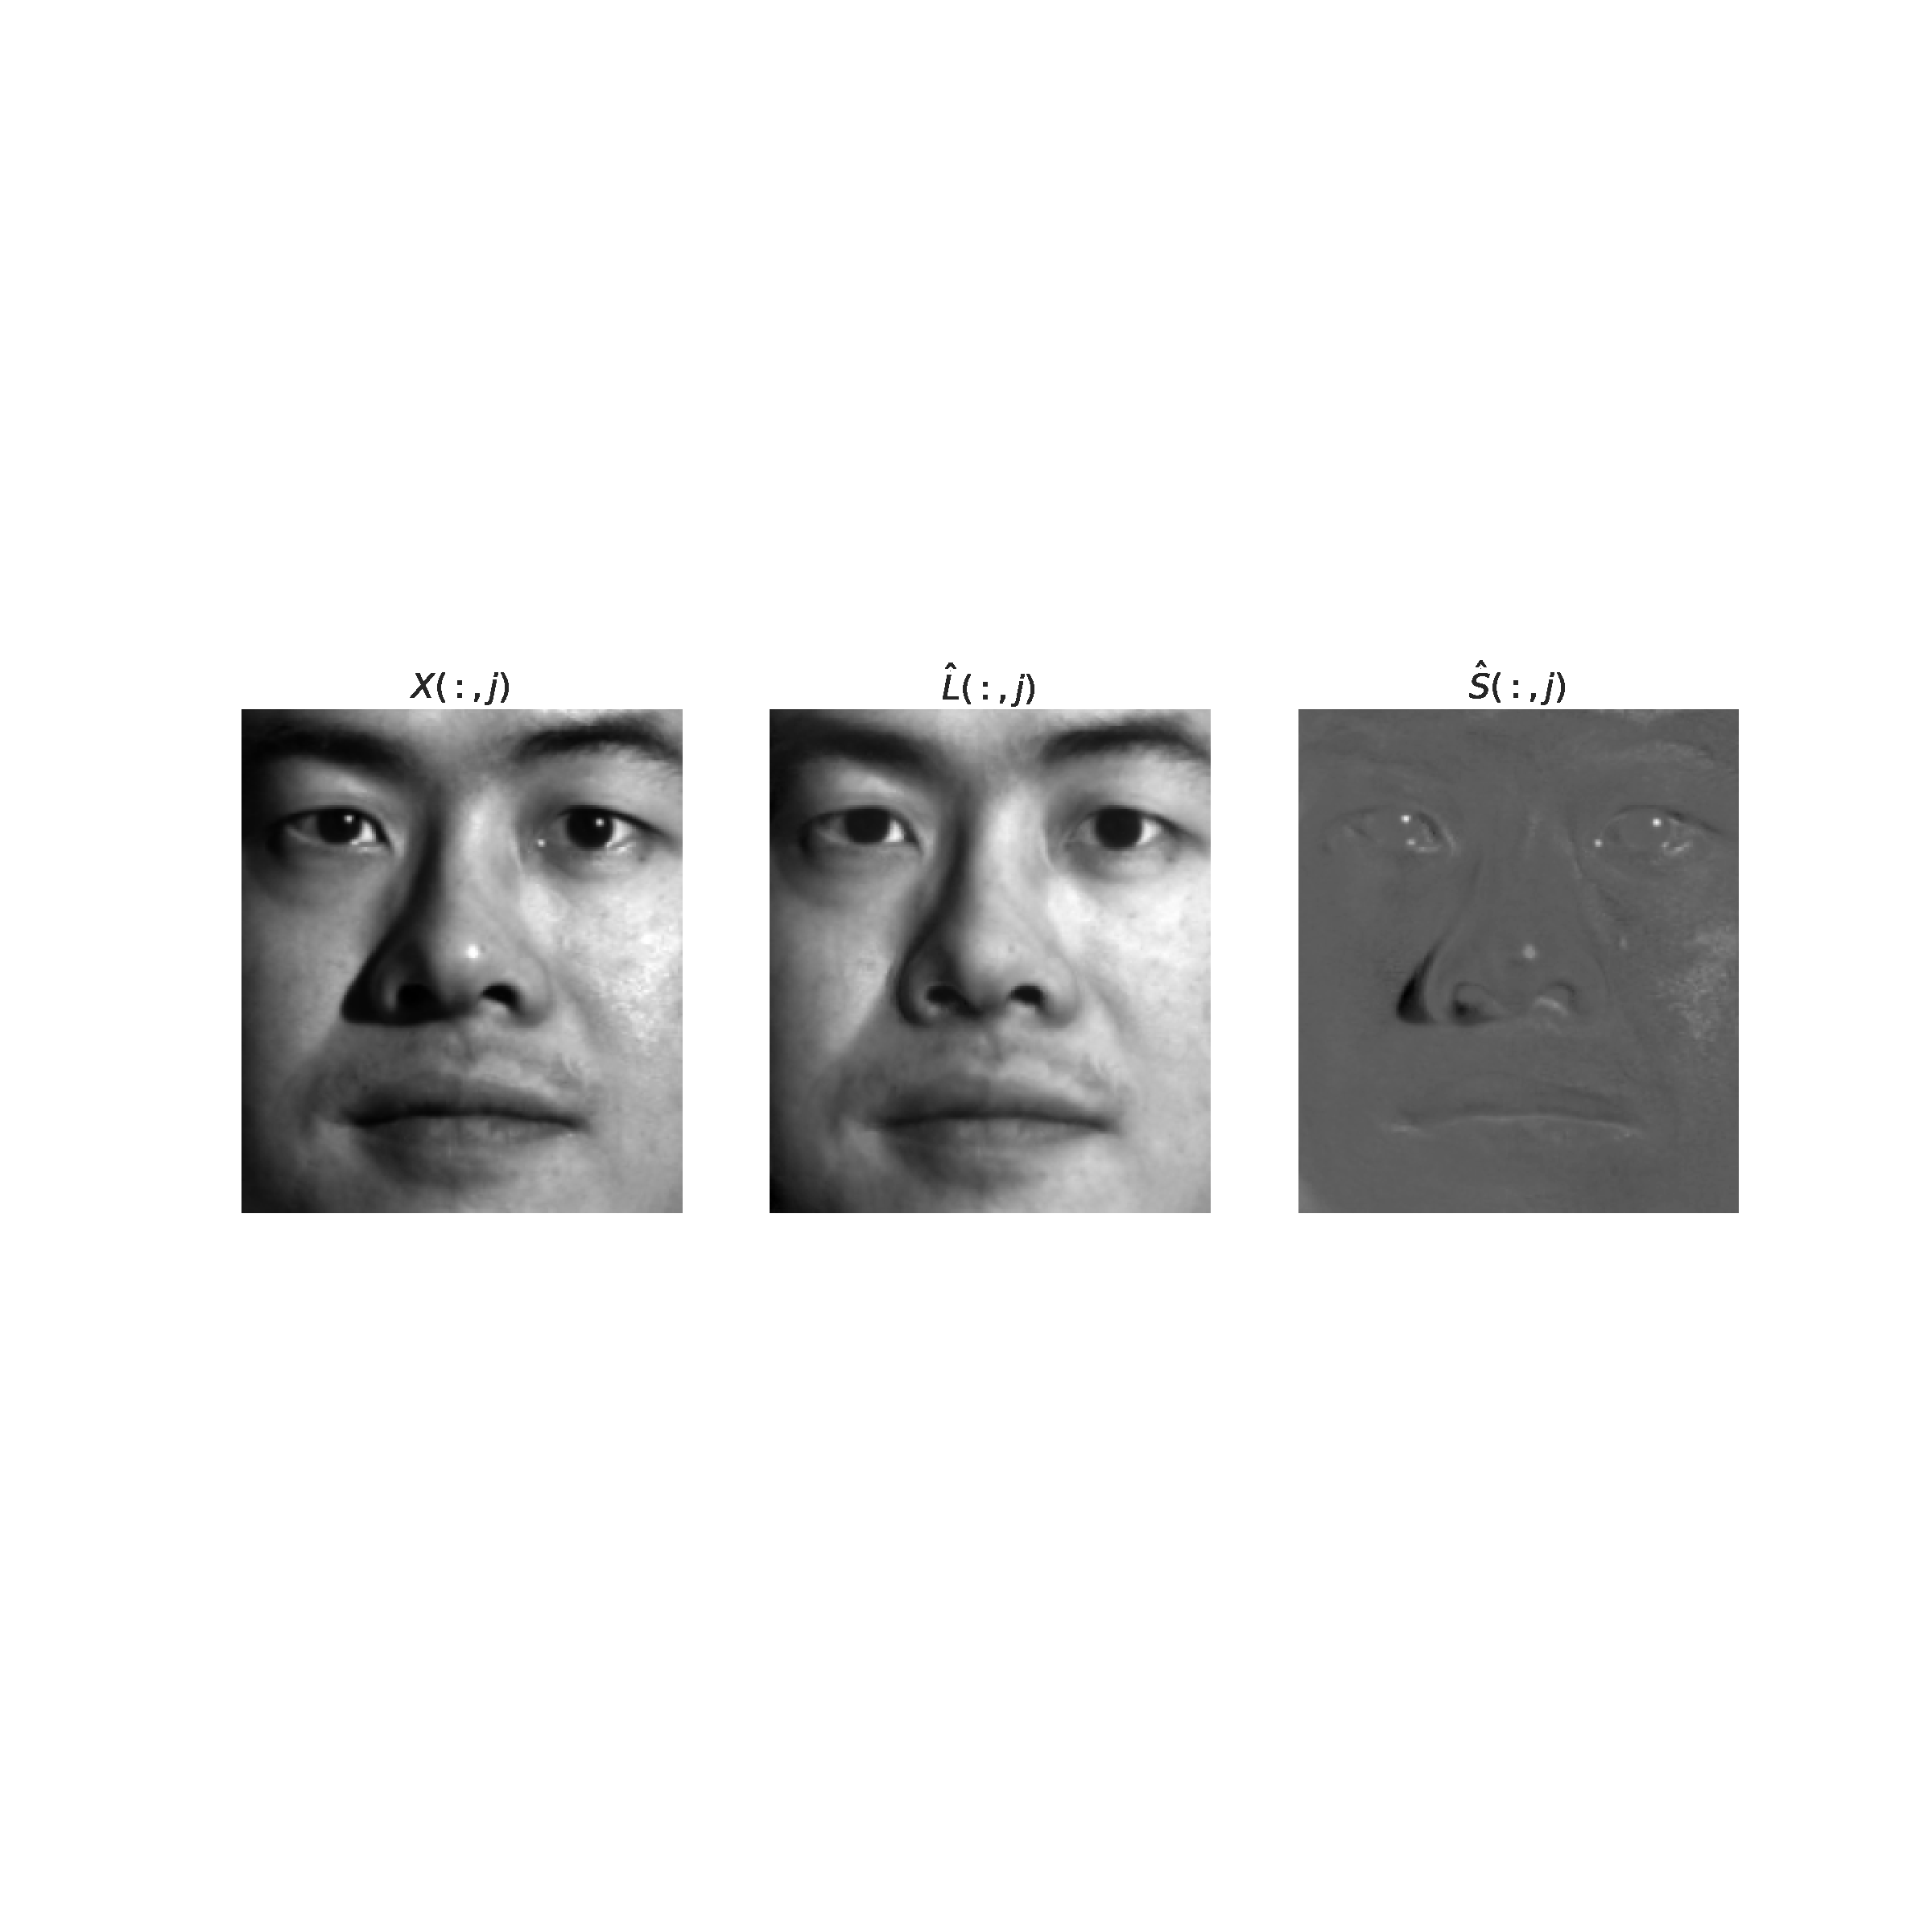
\includegraphics[width=1\linewidth]{image/Figure 6 Subgradient}
	\caption{Face Shadow Removal of Subgradient}
	\label{sub_face1}
\end{figure}

\subsection{A-IRLS Algorithm}
We set the iteration number equals to 100 to get $\boldsymbol{L}^{\star}=\boldsymbol{U}^{\star}\boldsymbol{V}^{\star\top}$ and we can see the loss appears to be decreasing with iteration as Figrue \ref{irls_face1}.
\begin{figure}[htbp]
	\centering
	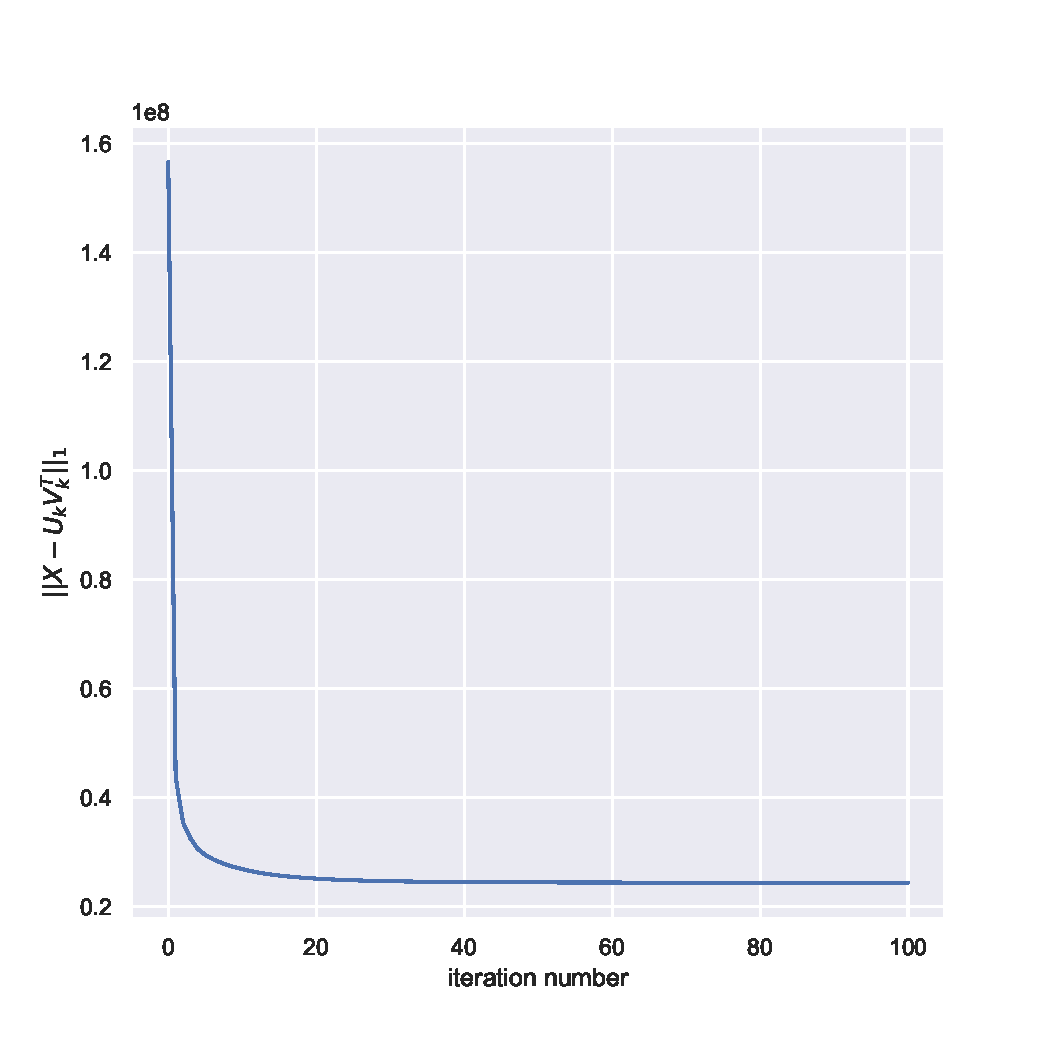
\includegraphics[width=0.6\linewidth]{image/Figure 7 A-IRLS}
	\caption{Iteration Process of A-IRLS in Face Image Data}
	\label{irls_face1}
\end{figure}

The results of face shadow removal are shown  as Figure \ref{irls_face2}. $\boldsymbol{X}$ is the original images, $\boldsymbol{\widehat{L}}$ is the processed images and $\boldsymbol{\widehat{S}}$ is the removed shadow. We can see the shadow are removed from the original image.

\begin{figure}[htbp]
	\centering
	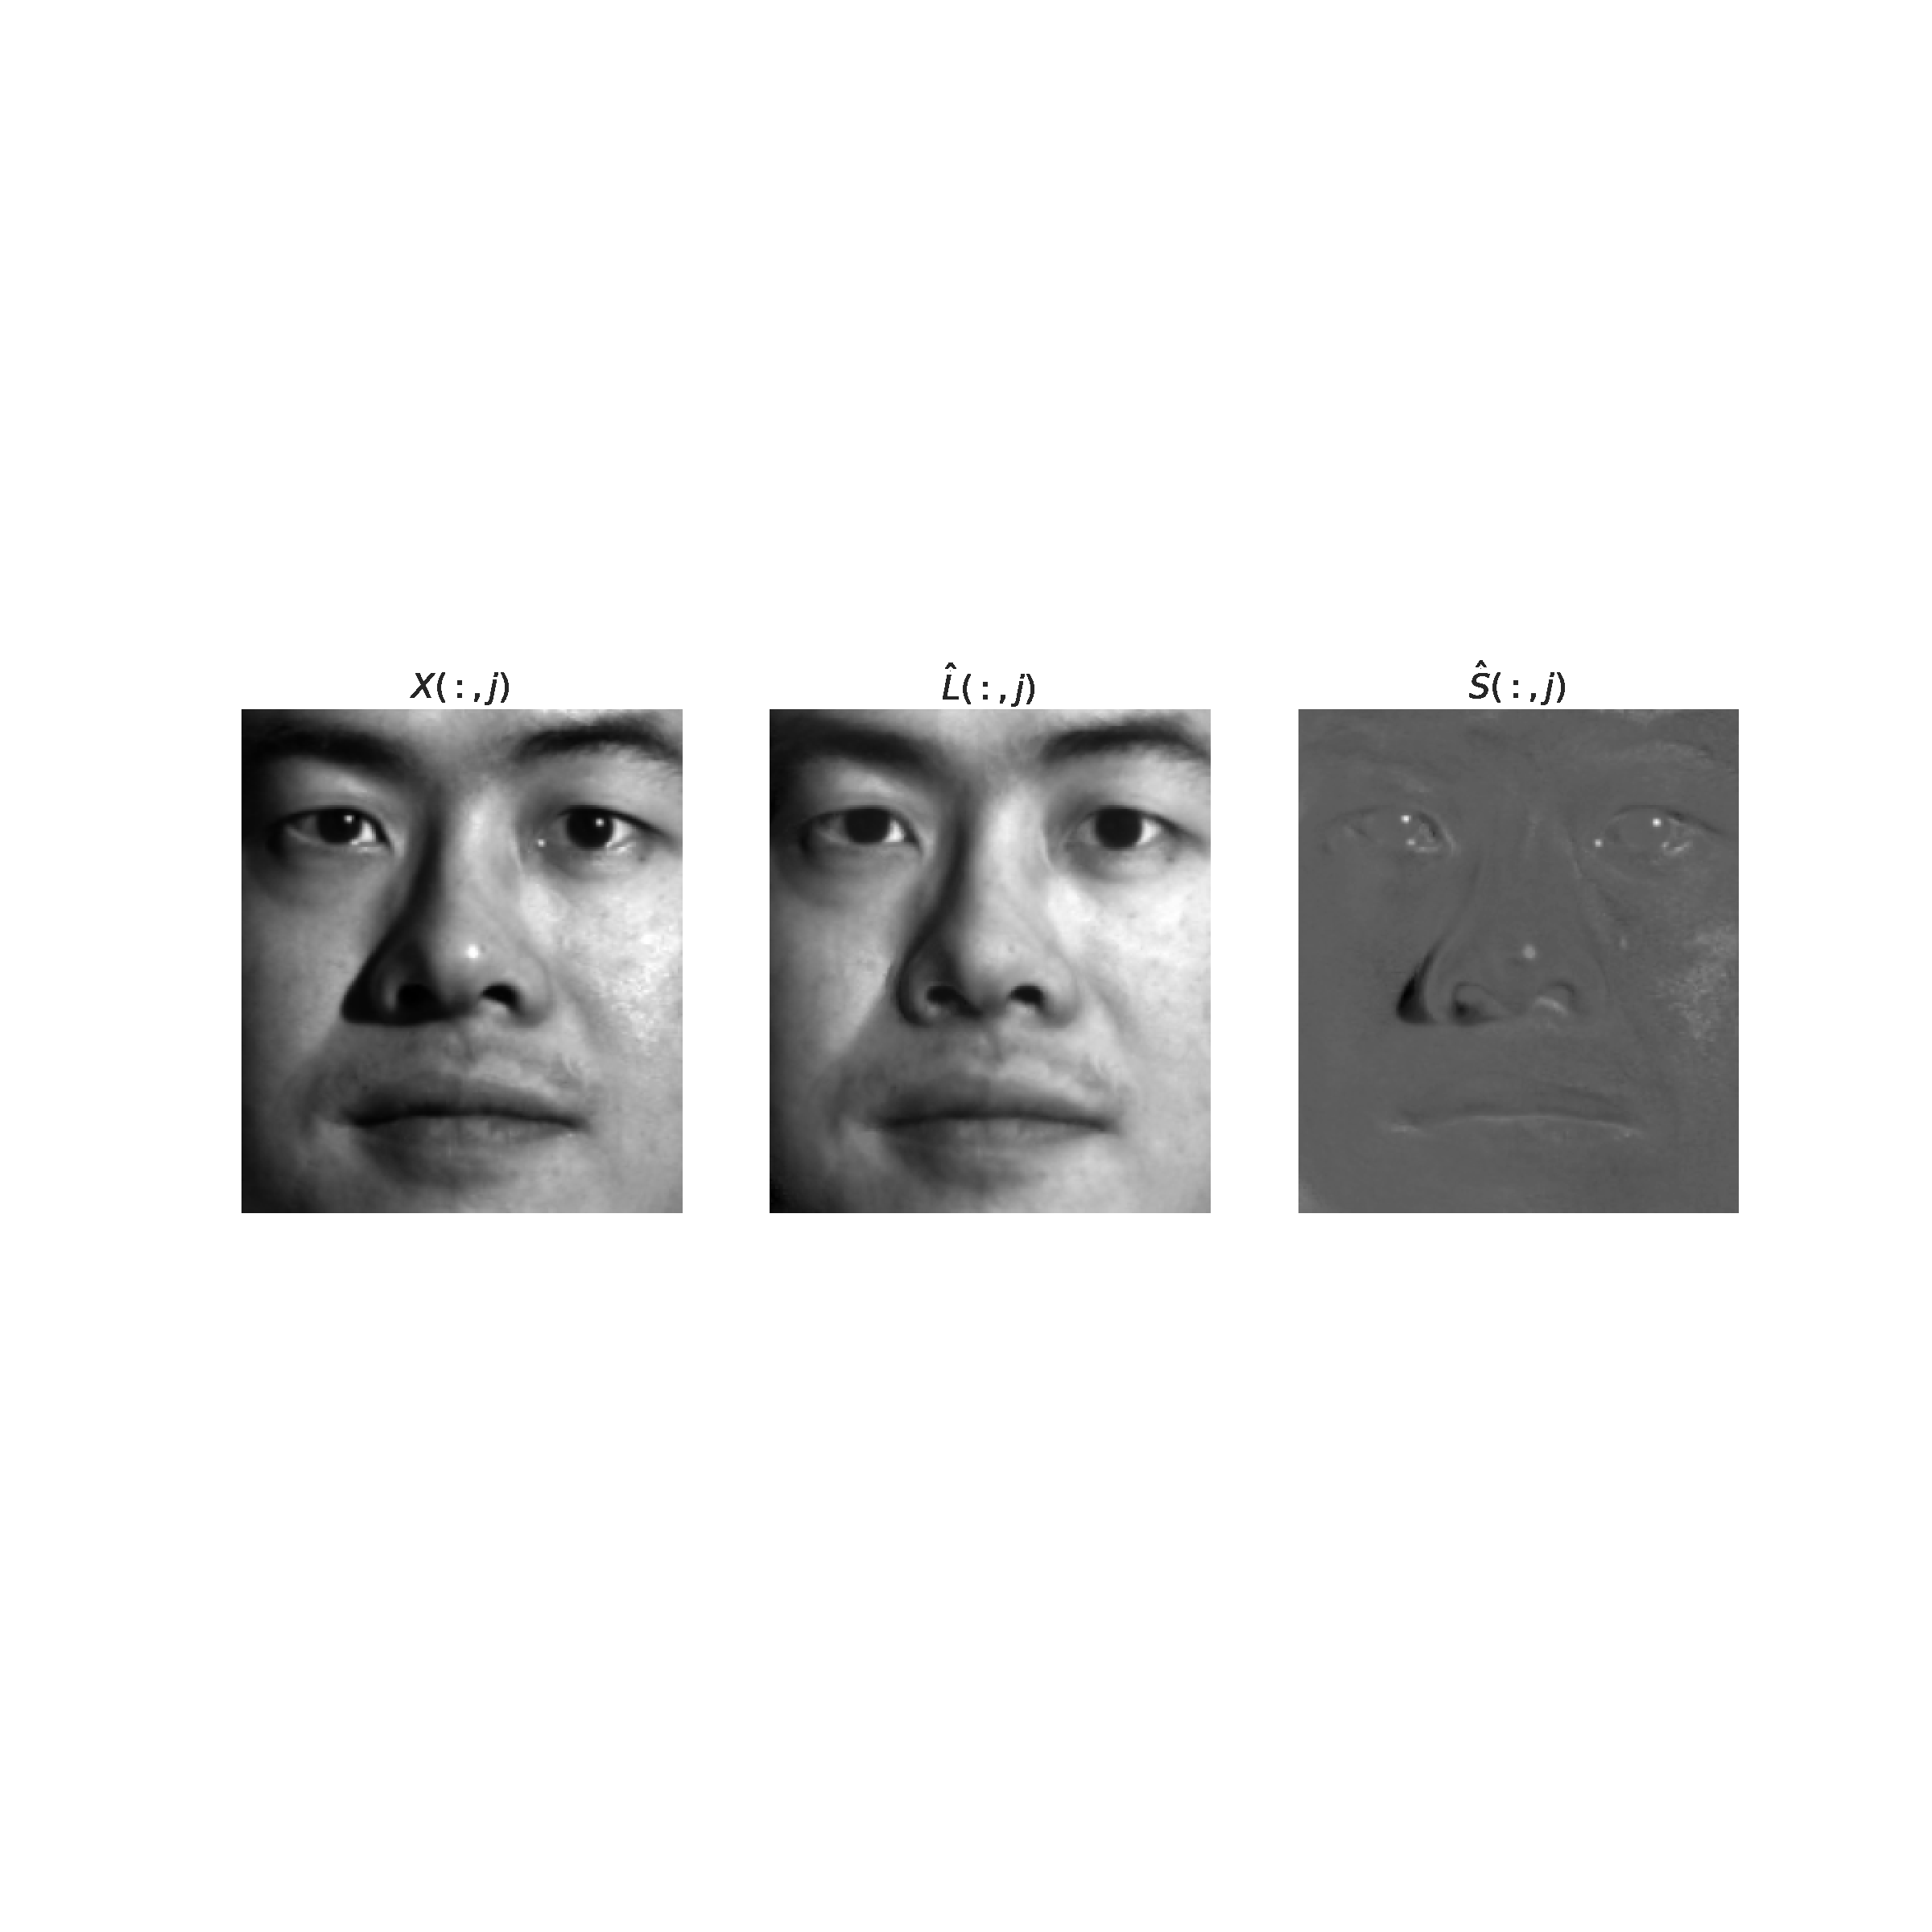
\includegraphics[width=1\linewidth]{image/Figure 8 A-IRLS}
	\caption{Face Shadow Removal of A-IRLS}
	\label{irls_face2}
\end{figure}


According to the figures shown above, the performance of both algorithms for face shadow removal are well while sub-gradient method needs more iterations to achieve similar result.

\section{Static Background Extraction}
In this part, we apply our algorithms to the escalator video dataset of a moving escalator and some pedestrians. The csv-format video is composed of 200 frames each with $130 \times 160$ pixels. Our goal is to split the video into non-static foreground and static background. 
The background has similar components as the original image, thus can be expressed by low rank matrices. Thus, the process can also be transformed into the minimization problem we have clarified above.

\subsection{Subgradient Method}
We set the iteration number equals to 2000 and the iteration process is similar as previous display of subgradient method. The loss still decreases rapidly in first 250 iterations and then fluctuates around a value in future iterations as in Figure \ref{sub_es1}.

\begin{figure}[htbp]
	\centering
	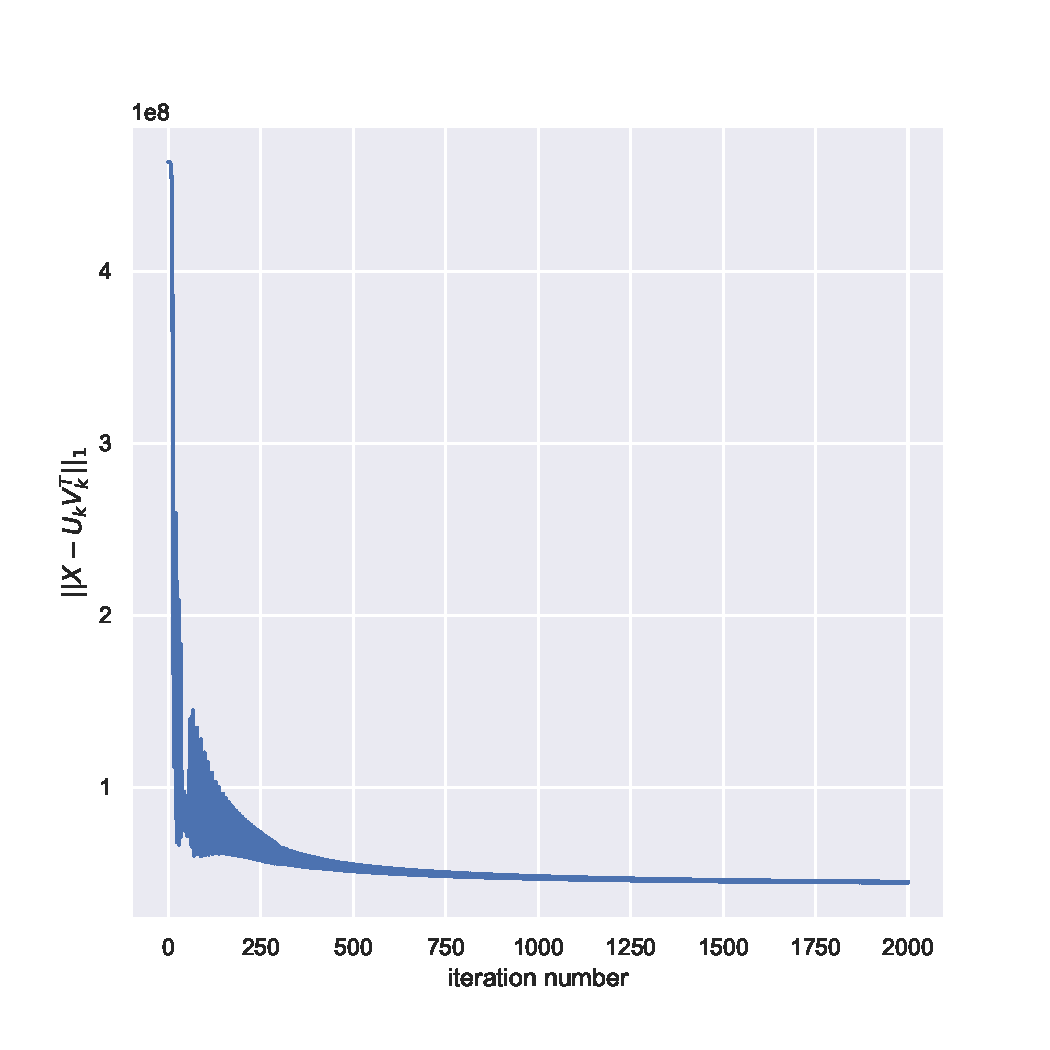
\includegraphics[width=0.6\linewidth]{image/Figure 9 Subgradient}
	\caption{Iteration Process of Subgradient in Escalator Data}
	\label{sub_es1}
\end{figure}

After implementation of algorithm, we can obtain $\boldsymbol{\widehat{L}}$ and $\boldsymbol{\widehat{S}}$. Each column of $\boldsymbol{X}$, $\boldsymbol{\widehat{L}}$ and $\boldsymbol{\widehat{S}}$ represents an image of original picture, estimated background and foreground respectively. Here is an example as Figure \ref{sub_es2}.

\begin{figure}[htbp]
	\centering
	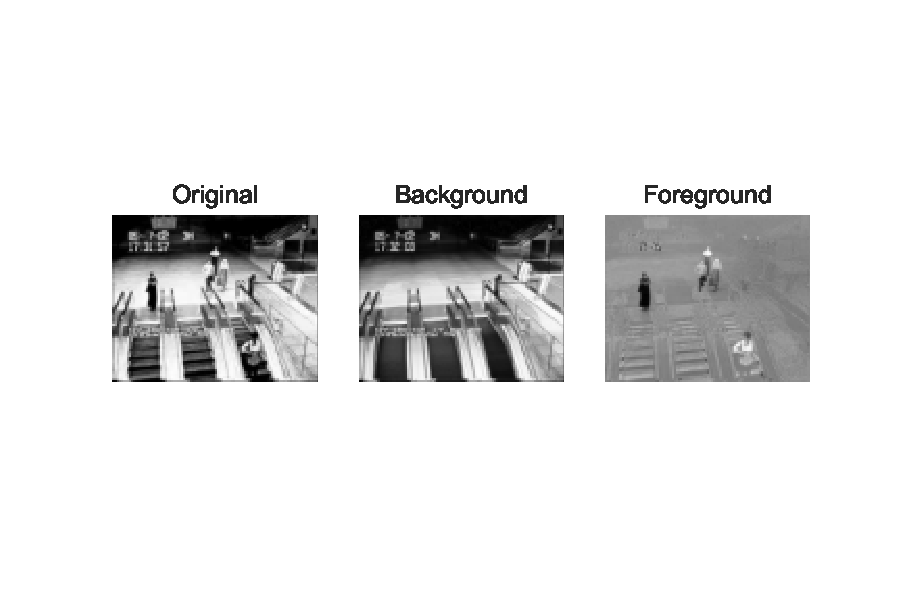
\includegraphics[width=1\linewidth]{image/Figure 10 Subgradient}
	\caption{Example of Static Background Extraction by Subgradient}
	\label{sub_es2}
\end{figure}

And by combining the 200 images together, we can obtain the whole video of background and foreground which is attached in the submitted folder.
\subsection{A-IRLS Algorithm}
We set the iteration number equals to 50 and the result comes as expected. The loss appears to be decreasing with iteration and we can see the process has the rise fluctuation in about $6^{th}$ iteration. The results are shown as Figure \ref{airls_es1}.

\begin{figure}[htbp]
	\centering
	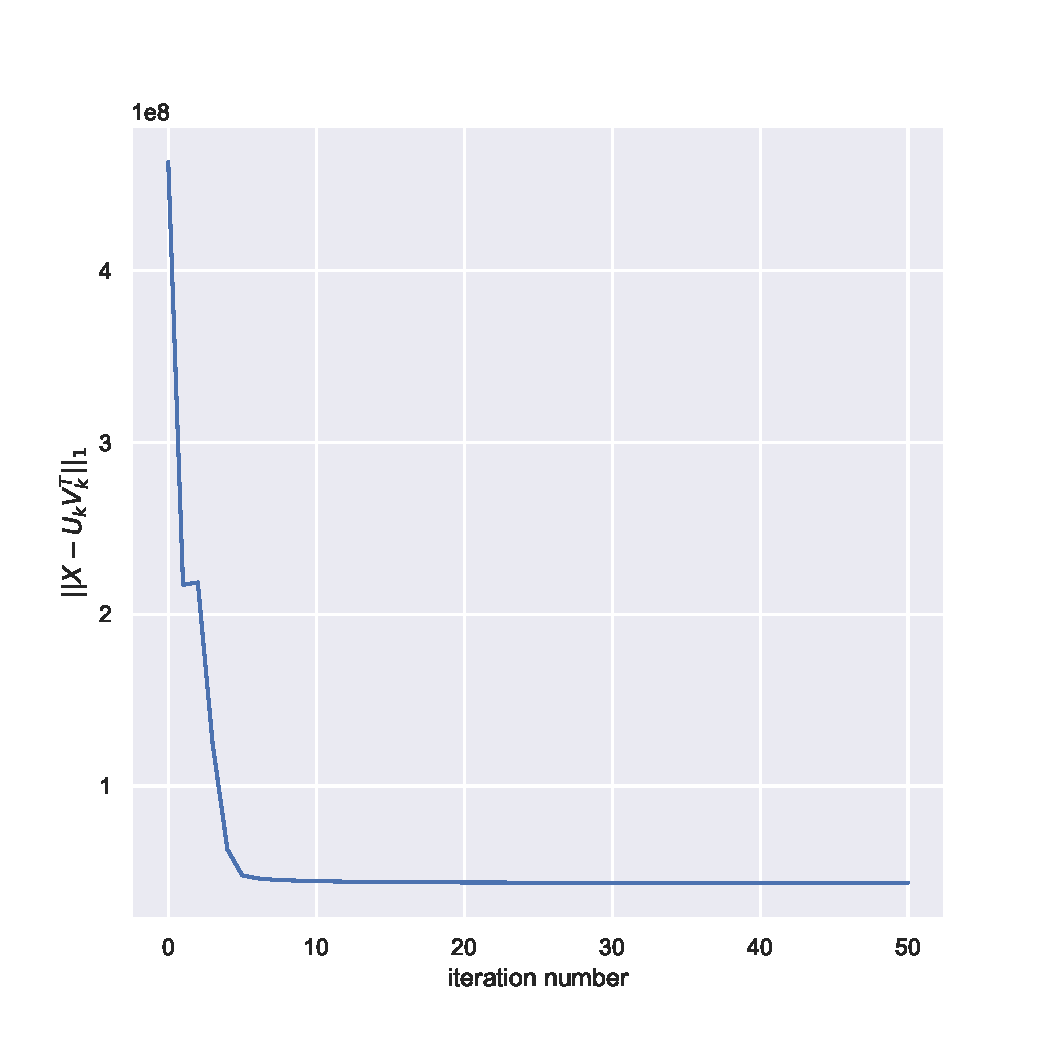
\includegraphics[width=0.6\linewidth]{image/Figure 11 A-IRLS}
	\caption{Iteration Process of A-IRLS in Escalator Data}
	\label{airls_es1}
\end{figure}

After implementation of algorithm, we can obtain $\boldsymbol{\widehat{L}}$ and $\boldsymbol{\widehat{S}}$. Each column of $\boldsymbol{X}$, $\boldsymbol{\widehat{L}}$ and $\boldsymbol{\widehat{S}}$ represents an image of original picture, estimated background and foreground respectively. Here is an example as Figure \ref{airls_es2}.
\begin{figure}[htbp]
	\centering
	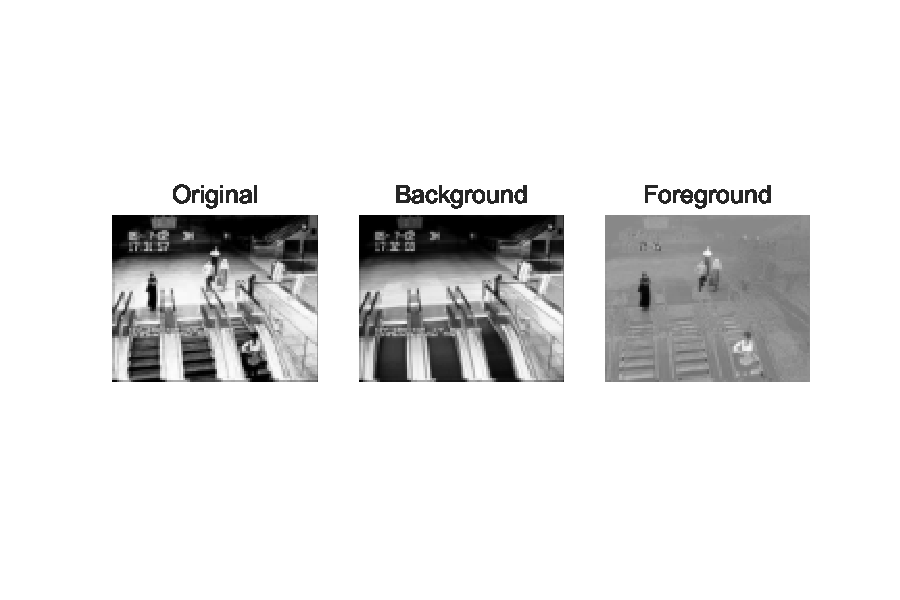
\includegraphics[width=1\linewidth]{image/Figure 12 A-IRLS}
	\caption{Example of Static Background Extraction by A-IRLS}
	\label{airls_es2}
\end{figure}

And by combining the 200 images together, we can obtain the whole video of background and foreground which is attached in the submitted folder.

\section{Conclusion}
In this report, we apply subgradient method and A-IRLS algorithm on three matrix factorization/PCA problems: artificial datasets, face shadow removal and Static Background Extraction. In the artificial dataset evaluation, we find out good sparsity is useful for our model; In the process of face shadow removal, we have successfully removed a proportion of shadow of original image. However, due to limited iteration number the results are not so perfect; In the problem of escalator video, we have divided background and foreground of each image of the video and then combined them as a new video.

Comparatively, both algorithms provide satisfactory performance while A-IRLS algorithm reaches a litter bit smaller error and converges in a much faster speed.

In the future model tuning and development, we may try different algorithms and increase the iteration numbers in the process of algorithms to get better performance and results. 


\bibliography{mybib}
\bibliographystyle{IEEEtran}
\section*{Appendix}
All the codes and supporting materials can be found in our github repository.
\end{document}
